% 18 variables in here:
% h_1 = 10.0, h_2 = 12.0, h_3 = 7.0, h_4 = 15.0, h_5 = 11.0, h_6 = 9.0, ux_1 = 0.0, ux_2 = 0.0, ux_3 = 0.0, ux_4 = 0.0, ux_5 = 0.0, ux_6 = 0.0, uy_1 = 0.0, uy_2 = 0.0, uy_3 = 0.0, uy_4 = 0.0, uy_5 = 0.0, uy_6 = 0.0
\begin{figure}[h!]
\centering
  \quad \subfloat[Error for the $x$ momentom for the first basis function. Heights are $h_2 = 12.0, h_3 = 7.0, h_4 = 15.0, h_5 = 11.0, h_6 = 9.0$, $h_1$ ranges from 8 to 12. All momentums are 0.] {
    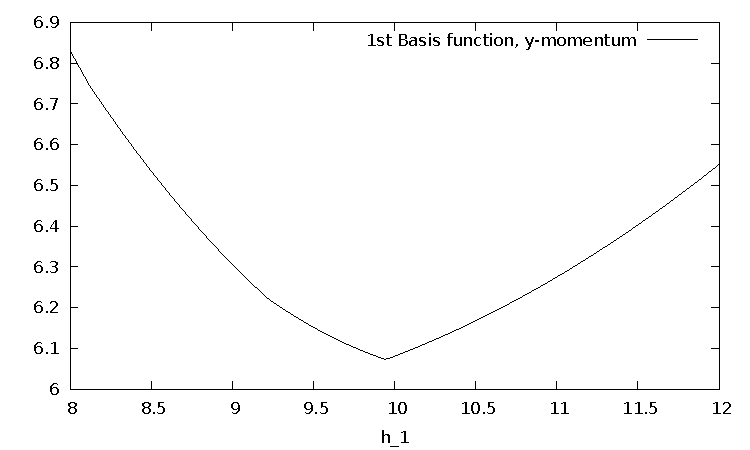
\includegraphics[scale=\zoomfactor]{{{ord2_magnitude_10_nonstd1/y_12.0_7.0_15.0_11.0_9.0_0.0_0.0_0.0_0.0_0.0_0.0_0.0_0.0_0.0_0.0_0.0_0.0f01}}}
  }
  \hspace{.5cm}
  \quad \subfloat[Error for the $x$ momentom for the fourth basis function. Heights are $h_2 = 12.0, h_3 = 7.0, h_4 = 15.0, h_5 = 11.0, h_6 = 9.0$, $h_1$ ranges from 8 to 12. All momentums are 0.] {
    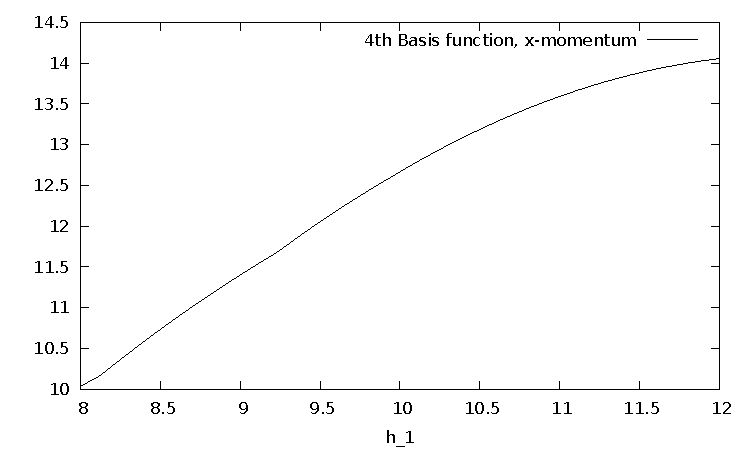
\includegraphics[scale=\zoomfactor]{{{ord2_magnitude_10_nonstd1/y_12.0_7.0_15.0_11.0_9.0_0.0_0.0_0.0_0.0_0.0_0.0_0.0_0.0_0.0_0.0_0.0_0.0f06}}}
  }
  % \quad \subfloat[] {
  %   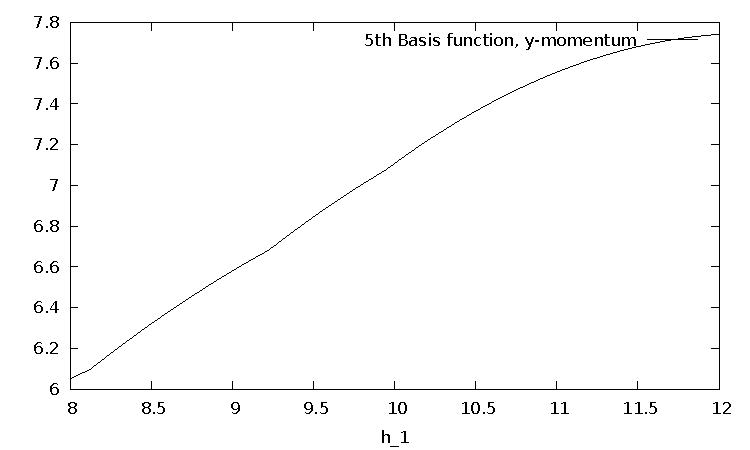
\includegraphics[scale=\zoomfactor]{{{ord2_magnitude_10_nonstd1/y_12.0_7.0_15.0_11.0_9.0_0.0_0.0_0.0_0.0_0.0_0.0_0.0_0.0_0.0_0.0_0.0_0.0f09}}}
  % }

  \quad \subfloat[Error for the $x$ momentom for the first basis function. Heights are $h_2 = 1002.0, h_3 = 997.0, h_4 = 1005.0, h_5 = 1001.0, h_6 = 999.0$, $h_1$ ranges from 998 to 1002. All momentums are 0.] {
    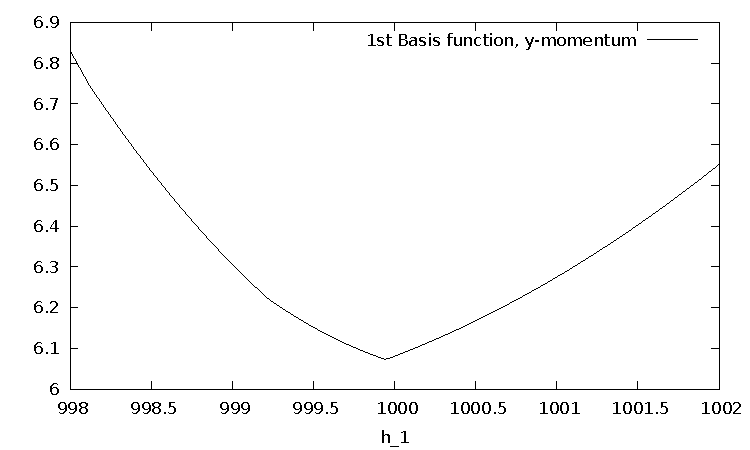
\includegraphics[scale=\zoomfactor]{{{ord2_magnitude_1000_nonstd1/y_1002.0_997.0_1005.0_1001.0_999.0_0.0_0.0_0.0_0.0_0.0_0.0_0.0_0.0_0.0_0.0_0.0_0.0f01}}}
  }
  \hspace{.5cm}
  \quad \subfloat[Error for the $x$ momentom for the fourth basis function. Heights are $h_2 = 1002.0, h_3 = 997.0, h_4 = 1005.0, h_5 = 1001.0, h_6 = 999.0$, $h_1$ ranges from 998 to 1002. All momentums are 0.] {
    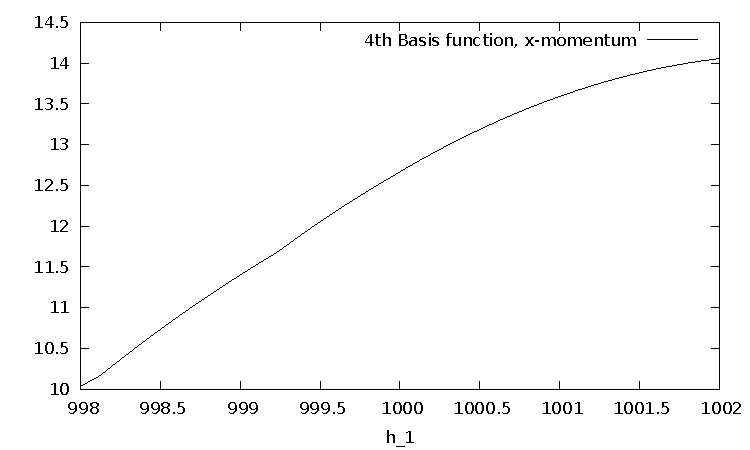
\includegraphics[scale=\zoomfactor]{{{ord2_magnitude_1000_nonstd1/y_1002.0_997.0_1005.0_1001.0_999.0_0.0_0.0_0.0_0.0_0.0_0.0_0.0_0.0_0.0_0.0_0.0_0.0f06}}}
  }
  % \quad \subfloat[] {
  %   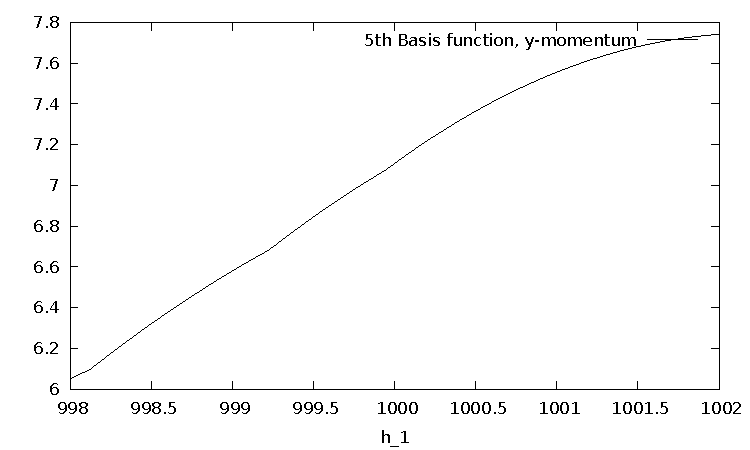
\includegraphics[scale=\zoomfactor]{{{ord2_magnitude_1000_nonstd1/y_1002.0_997.0_1005.0_1001.0_999.0_0.0_0.0_0.0_0.0_0.0_0.0_0.0_0.0_0.0_0.0_0.0_0.0f09}}}
  % }
\caption{Comparison of errors for different orders of magnitude concerning height values. All momentums are left 0. Error plots are the same for the different orders of magnitude examined in this scenario.}
\label{fig:ord2_magnitude_comparison_momentums}
\end{figure}

%%% Local Variables:
%%% TeX-master: "../results.tex"
%%% End:
